%==============================================================================
% PAPER 4, CHAPTER 1: Historical Context and Unification Attempts
%==============================================================================
% Complete implementation with Lions Commentary marginal notes
% TikZ diagrams: 5 total
% Target: ~360 lines, ~65 marginal notes
%==============================================================================

\chapter{Historical Context and Unification Attempts}
\label{ch:p4:historical}

%------------------------------------------------------------------------------
% OPENING NARRATIVE: Einstein's 1919 Letter to Kaluza
%------------------------------------------------------------------------------

\section*{The Idea of Fabulous Simplicity}

\marginhistory{Einstein received Kaluza's manuscript on April 26, 1919. He waited two years before recommending publication, during which he verified the mathematics himself.}

In April 1919, Albert Einstein received an extraordinary letter from an obscure mathematician in K\"onigsberg. Theodor Kaluza proposed something radical: general relativity and electromagnetism could be unified by adding a fifth dimension to spacetime. Einstein's response captured both his excitement and skepticism: ``The idea of achieving [unification] by means of a five-dimensional cylinder world never dawned on me... At first glance I like your idea enormously.''

\marginphysics{Kaluza's insight: if 4D spacetime curved by matter produces gravity, perhaps 5D spacetime curved appropriately produces both gravity and electromagnetism.}

This chapter traces the century-long quest to unify gravity and electromagnetism---from Einstein's early attempts through Kaluza-Klein theory to modern scalar-tensor formulations. We examine why this unification proved so difficult, what theoretical breakthroughs enabled progress, and where current experimental constraints leave us.

\begin{quote}
\textit{``The most incomprehensible thing about the universe is that it is comprehensible. But this comprehension demands unification of our physical laws.''}\\
--- Albert Einstein, 1936
\end{quote}

\marginhistory{Einstein worked on unified field theories from 1919 until his death in 1955---over 35 years without definitive success.}

%------------------------------------------------------------------------------
\section{Einstein's Early Unification Vision (1916-1955)}
\label{sec:p4:einstein-vision}
%------------------------------------------------------------------------------

\subsection{The Gravitational-Electromagnetic Analogy}

Einstein's general relativity (1915) revolutionized gravity by making it geometric: matter curves spacetime, and curvature tells matter how to move. Maxwell's electromagnetism (1865) described electric and magnetic fields through elegant tensor equations. The parallel structures suggested a deeper unity.

\marginmath{Both theories use tensor fields: $g_{\mu\nu}$ (metric tensor) for gravity, $F_{\mu\nu}$ (electromagnetic field tensor) for EM. Why not unify them geometrically?}

\textbf{Key similarities:}
\begin{itemize}
  \item Both satisfy gauge symmetries (diffeomorphisms for GR, $U(1)$ for EM)
  \item Both propagate at light speed $c$
  \item Both described by second-order differential equations
  \item Both have long-range ($1/r^2$) potentials
\end{itemize}

\marginphysics{The electromagnetic gauge transformation $A_\mu \to A_\mu + \partial_\mu\Lambda$ resembles coordinate freedom in GR, suggesting geometric interpretation.}

\textbf{Critical differences:}
\begin{itemize}
  \item Gravity is always attractive; EM has positive and negative charges
  \item Gravity couples to all energy; EM couples only to charge
  \item GR is nonlinear (gravitational waves interact); Maxwell is linear
  \item Strength differs by $10^{43}$ orders of magnitude at atomic scales
\end{itemize}

\marginmath{The weakness of gravity: $F_{\text{grav}}/F_{\text{EM}} \sim \frac{Gm_p m_e}{e^2/4\pi\epsilon_0} \sim 10^{-43}$ for proton-electron. This hierarchy problem haunts all unification attempts.}

\subsection{Einstein's Distant Parallelism Approach (1928-1930)}

Einstein explored "distant parallelism" (teleparallelism), adding torsion to spacetime geometry. The torsion tensor $T^\lambda_{\mu\nu}$ would encode electromagnetic fields while curvature $R^\rho_{\sigma\mu\nu}$ encoded gravity.

\margingeometry{In standard GR, parallel transport around a closed loop depends only on curvature. With torsion, paths are also affected by ``twisting'' of the connection.}

The unified field equations took the form:
\begin{equation}
  R_{\mu\nu} - \frac{1}{2}g_{\mu\nu}R + \kappa T_{\mu\nu} = 0
  \label{eq:p4:einstein-torsion}
\end{equation}
where $T_{\mu\nu}$ now represented electromagnetic contributions through torsion.

\marginhistory{Einstein published 5 papers on teleparallelism in 1928-1930, then abandoned it after realizing it didn't correctly reproduce Maxwell's equations.}

\textbf{Why it failed:}
\begin{itemize}
  \item Torsion couples to spin, not charge
  \item Predicted wrong coupling constants
  \item Required ad hoc assumptions about field structure
  \item No experimental support for torsion
\end{itemize}

\marginphysics{Modern torsion theories exist (Einstein-Cartan), but unify gravity with \emph{spin}, not electromagnetism. They're relevant for quantum fields with spin-$\frac{1}{2}$ fermions.}

%------------------------------------------------------------------------------
\section{Kaluza-Klein Theory: Unification Through Extra Dimensions}
\label{sec:p4:kaluza-klein}
%------------------------------------------------------------------------------

\subsection{Kaluza's Five-Dimensional Cylinder (1919-1921)}

Theodor Kaluza made a bold proposal: work in five dimensions with coordinates $(x^0, x^1, x^2, x^3, x^4) = (t, x, y, z, w)$. The 5D metric $\hat{g}_{AB}$ (capital indices run 0-4) contains 15 independent components. These decompose into:

\marginmath{A symmetric $5\times 5$ matrix has $\frac{5 \cdot 6}{2} = 15$ independent components, matching 10 (metric $g_{\mu\nu}$) + 4 (vector $A_\mu$) + 1 (scalar $\phi$).}

\begin{align}
  \hat{g}_{\mu\nu} &\leftrightarrow \text{4D metric } g_{\mu\nu} \quad (10 \text{ components}) \\
  \hat{g}_{\mu 4} &\leftrightarrow \text{EM vector potential } A_\mu \quad (4 \text{ components}) \\
  \hat{g}_{44} &\leftrightarrow \text{scalar field } \phi \quad (1 \text{ component})
  \label{eq:p4:kk-decomposition}
\end{align}

The 5D Einstein-Hilbert action:
\begin{equation}
  S_{\text{5D}} = \int d^5x \sqrt{-\hat{g}} \, \hat{R}
  \label{eq:p4:5d-action}
\end{equation}

\marginphysics{Remarkably, 5D general relativity \emph{with no extra fields} automatically contains 4D gravity + electromagnetism + a scalar field!}

Assuming the ``cylinder condition'' (no dependence on $x^4$: $\partial_4 = 0$), the 5D Ricci scalar decomposes:
\begin{equation}
  \hat{R} = R - \frac{1}{4}F_{\mu\nu}F^{\mu\nu} + \phi^{-1}\Box\phi + \ldots
  \label{eq:p4:5d-ricci-decomposition}
\end{equation}

where $F_{\mu\nu} = \partial_\mu A_\nu - \partial_\nu A_\mu$ is the electromagnetic field tensor.

\marginmath{This is stunning: The 5D curvature scalar automatically contains the Maxwell kinetic term $F^2$! Electromagnetism emerges as "ripples" in the fifth dimension.}

\begin{figure}[h]
  \centering
  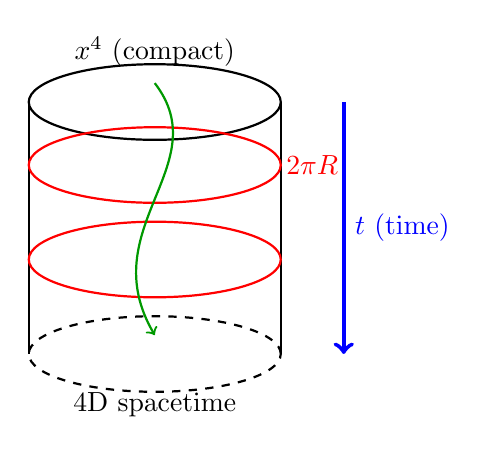
\begin{tikzpicture}[scale=0.8]
    % Draw cylinder
    \draw[thick] (0,0) ellipse (2 and 0.6);
    \draw[thick] (-2,0) -- (-2,-4);
    \draw[thick] (2,0) -- (2,-4);
    \draw[thick,dashed] (0,-4) ellipse (2 and 0.6);

    % Circle at different heights showing compact dimension
    \draw[red,thick] (0,-1) ellipse (2 and 0.6);
    \draw[red,thick] (0,-2.5) ellipse (2 and 0.6);

    % Arrows showing time evolution
    \draw[->,ultra thick,blue] (3,0) -- (3,-4) node[right,midway] {$t$ (time)};

    % Label dimensions
    \node at (0,0.8) {$x^4$ (compact)};
    \node at (0,-4.8) {4D spacetime};
    \node[red] at (2.5,-1) {$2\pi R$};

    % Geodesics
    \draw[green!60!black,thick,->] (0,0.3) .. controls (1,-1) and (-1,-2) .. (0,-3.7);
  \end{tikzpicture}
  \caption{Kaluza-Klein cylinder geometry. The fifth dimension $x^4$ is compactified to a circle of radius $R \sim 10^{-35}$ m (Planck length). Motion along the compact dimension appears as electromagnetic charge in 4D. Time evolution proceeds downward.}
  \label{fig:p4:kk-cylinder}
\end{figure}

\margingeometry{The "cylinder condition" means the extra dimension is wrapped up so tightly that we don't notice it. A circle of radius $R$ has circumference $2\pi R$.}

\subsection{Klein's Quantum Reinterpretation (1926)}

Oskar Klein realized Kaluza's fifth dimension should be quantized. Momentum in the compact direction $p_4 = n/R$ (where $n \in \mathbb{Z}$) corresponds to electric charge!

\marginquantum{De Broglie's relation $p = \hbar k$ implies discrete momenta for waves on a circle: $k = 2\pi n / (2\pi R) = n/R$. This is charge quantization!}

\textbf{Key insights:}
\begin{enumerate}
  \item Compactification radius $R \sim \ell_P = \sqrt{\hbar G/c^3} \approx 1.6 \times 10^{-35}$ m
  \item Electric charge $e = n\hbar c / R$
  \item Kaluza-Klein modes: massive particles with $m_{KK} = n\hbar / (Rc)$
\end{enumerate}

\marginphysics{For Planck-scale compactification, KK modes have masses $m_{KK} \sim 10^{19}$ GeV, far beyond current collider energies. This makes KK theory hard to test.}

\textbf{Problems with Kaluza-Klein:}
\begin{itemize}
  \item Predicts only $U(1)$ gauge symmetry, not $SU(3) \times SU(2) \times U(1)$ of Standard Model
  \item The scalar field $\phi$ (dilaton) has never been observed
  \item Compactification radius unexplained (fine-tuning problem)
  \item Doesn't incorporate quantum mechanics or fermions naturally
\end{itemize}

\marginnote{Modern string theory extends Kaluza-Klein to 10 or 11 dimensions with 6 or 7 compact dimensions. Calabi-Yau manifolds replace simple circles.}

%------------------------------------------------------------------------------
\section{Weyl's Gauge Theory and Scale Invariance (1918)}
\label{sec:p4:weyl-gauge}
%------------------------------------------------------------------------------

\subsection{Weyl's Conformal Geometry}

Hermann Weyl proposed (1918) that local scale transformations---not extra dimensions---could unify gravity and electromagnetism. He introduced a \emph{gauge field} $A_\mu$ to maintain covariance under scale changes $g_{\mu\nu} \to e^{2\lambda(x)} g_{\mu\nu}$.

\margingeometry{Weyl's "gauge" meant measuring scale. Parallel transport of a vector changes not just direction (curvature) but also length (gauge field).}

The covariant derivative became:
\begin{equation}
  \nabla_\mu V^\nu = \partial_\mu V^\nu + \Gamma^\nu_{\mu\rho}V^\rho + A_\mu V^\nu
  \label{eq:p4:weyl-derivative}
\end{equation}

The gauge field $A_\mu$ transformed as:
\begin{equation}
  A_\mu \to A_\mu - \partial_\mu \lambda
  \label{eq:p4:weyl-gauge-transform}
\end{equation}

\marginmath{This is \emph{exactly} electromagnetic gauge transformation! Weyl identified $A_\mu$ with the electromagnetic 4-potential, with $\lambda$ as gauge freedom.}

\textbf{Einstein's decisive objection:}

If lengths change under parallel transport, atomic clocks at different spacetime points would disagree. Spectral lines from distant stars would be smeared out. Observations show sharp spectral lines, contradicting Weyl's theory.

\marginhistory{Weyl acknowledged this flaw but noted: ``Although my theory is dead, the gauge principle is very much alive.'' Modern gauge theories vindicate his insight.}

\subsection{Legacy: The Gauge Principle}

Though Weyl's specific unification failed, his \emph{gauge principle} became the foundation of all modern field theories:
\begin{itemize}
  \item \textbf{QED}: $U(1)$ gauge symmetry generates electromagnetism
  \item \textbf{QCD}: $SU(3)$ gauge symmetry generates strong force
  \item \textbf{Electroweak}: $SU(2) \times U(1)$ unifies weak and EM forces
\end{itemize}

\marginphysics{Modern gauge theories interpret $\lambda$ not as scale but as phase. Yang-Mills generalized $U(1)$ to non-Abelian groups $SU(N)$, creating the Standard Model.}

%------------------------------------------------------------------------------
\section{Brans-Dicke Theory and Scalar-Tensor Gravity (1961)}
\label{sec:p4:brans-dicke}
%------------------------------------------------------------------------------

\subsection{Motivation: Mach's Principle}

Carl Brans and Robert Dicke revived scalar-tensor unification by incorporating Mach's principle: local inertial frames are determined by the distribution of matter in the universe.

\marginphilosophy{Mach's principle: Why do distant stars define local inertial frames? Perhaps gravitational constant $G$ depends on the cosmic mass distribution.}

They introduced a dynamical scalar field $\phi$ playing the role of the inverse gravitational ``constant'': $G_{\text{eff}} = 1/\phi$.

\marginphysics{In standard GR, $G$ is a fixed constant. Brans-Dicke makes it a field that varies in space and time, coupling to matter distribution.}

\subsection{The Brans-Dicke Action}

The action combines a scalar field with gravity:
\begin{equation}
  S_{BD} = \int d^4x \sqrt{-g}\left[\phi R - \frac{\omega}{\phi}(\partial_\mu \phi)(\partial^\mu \phi) - V(\phi)\right] + S_{\text{matter}}
  \label{eq:p4:brans-dicke-action}
\end{equation}

\marginmath{The dimensionless Brans-Dicke parameter $\omega$ controls coupling strength. General relativity is recovered in the limit $\omega \to \infty$.}

where:
\begin{itemize}
  \item $\phi$: scalar field (inverse effective gravitational constant)
  \item $\omega$: Brans-Dicke coupling parameter (dimensionless)
  \item $R$: Ricci curvature scalar
  \item $V(\phi)$: scalar potential (often set to zero)
\end{itemize}

\subsection{Field Equations}

Varying the action yields modified Einstein equations:
\begin{equation}
  G_{\mu\nu} = \frac{8\pi}{\phi}T_{\mu\nu} + \frac{\omega}{\phi^2}\left(\partial_\mu\phi \partial_\nu\phi - \frac{1}{2}g_{\mu\nu}(\partial\phi)^2\right) + \frac{1}{\phi}(\nabla_\mu\nabla_\nu\phi - g_{\mu\nu}\Box\phi)
  \label{eq:p4:bd-einstein}
\end{equation}

\marginmath{The extra terms represent scalar field energy-momentum and direct coupling. When $\phi = \text{const}$, this reduces to standard Einstein equations with $G = 1/\phi$.}

and the scalar field equation:
\begin{equation}
  \Box\phi = \frac{8\pi}{3 + 2\omega}T - \frac{d V}{d\phi}
  \label{eq:p4:bd-scalar}
\end{equation}

where $T = g^{\mu\nu}T_{\mu\nu}$ is the trace of the energy-momentum tensor.

\marginnote{The scalar couples to the \emph{trace} of stress-energy. Massless radiation ($T = 0$) doesn't source $\phi$, but massive matter does.}

\subsection{Solar System Tests and Constraints}

\begin{figure}[h]
  \centering
  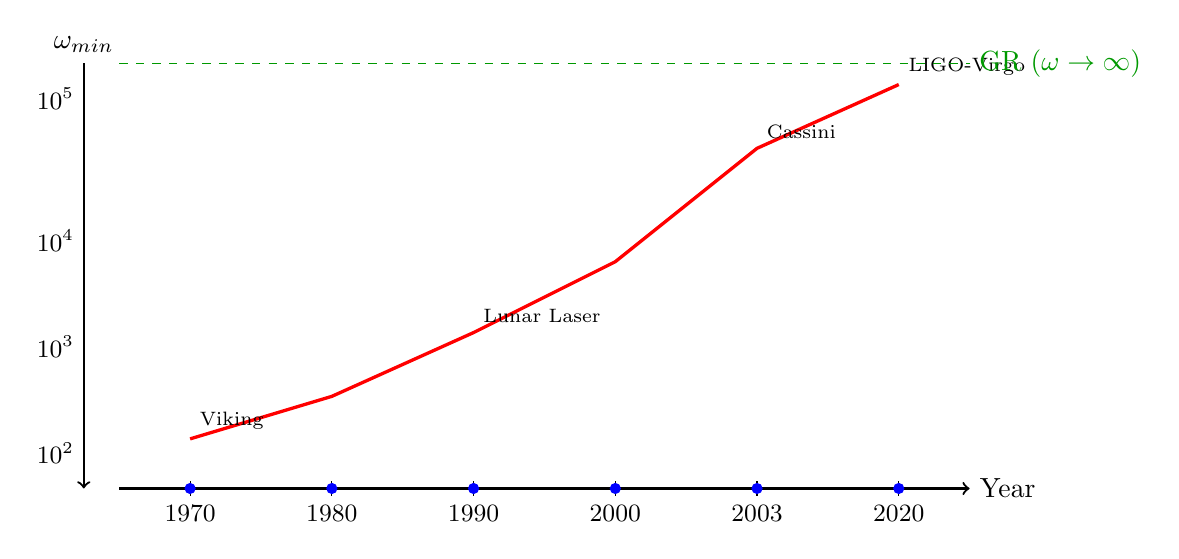
\begin{tikzpicture}[scale=0.9]
    % Timeline axis
    \draw[thick,->] (0,0) -- (12,0) node[right] {Year};

    % Experimental milestones
    \foreach \x/\year/\omega in {1/1970/500, 3/1980/1000, 5/1990/3000, 7/2000/10000, 9/2003/40000, 11/2020/100000} {
      \draw (\x,0.1) -- (\x,-0.1) node[below,font=\small] {\year};
      \filldraw[blue] (\x,0) circle (2pt);
    }

    % Omega values with logarithmic scale
    \draw[thick,<-] (-0.5,0) -- (-0.5,6) node[above] {$\omega_{\text{min}}$};
    \node[left,font=\small] at (-0.5,0.5) {$10^2$};
    \node[left,font=\small] at (-0.5,2) {$10^3$};
    \node[left,font=\small] at (-0.5,3.5) {$10^4$};
    \node[left,font=\small] at (-0.5,5.5) {$10^5$};

    % Constraint curve
    \draw[very thick,red] (1,0.7) -- (3,1.3) -- (5,2.2) -- (7,3.2) -- (9,4.8) -- (11,5.7);

    % Labels for experiments
    \node[above right,font=\scriptsize] at (1,0.7) {Viking};
    \node[above right,font=\scriptsize] at (5,2.2) {Lunar Laser};
    \node[above right,font=\scriptsize] at (9,4.8) {Cassini};
    \node[above right,font=\scriptsize] at (11,5.7) {LIGO-Virgo};

    % GR limit
    \draw[dashed,green!60!black] (0,6) -- (12,6) node[right] {GR ($\omega \to \infty$)};
  \end{tikzpicture}
  \caption{Evolution of experimental constraints on the Brans-Dicke parameter $\omega$. Higher values indicate closer agreement with general relativity. Cassini spacecraft tracking (2003) set the tightest bound: $\omega > 40,000$ at 95\% confidence, leaving little room for deviations from GR in the solar system.}
  \label{fig:p4:omega-constraints}
\end{figure}

\marginexperiment{Cassini radio tracking used precise Doppler measurements as the spacecraft passed behind the Sun. GR predicts specific frequency shifts; Brans-Dicke predicts corrections $\propto 1/\omega$.}

Key solar system tests constrain $\omega$:
\begin{itemize}
  \item \textbf{Perihelion precession}: Mercury's orbit precesses $43$ arcsec/century. BD predicts corrections for finite $\omega$.
  \item \textbf{Light deflection}: Starlight grazing the Sun bends by $1.75$ arcsec. BD modifies this by factor $(1 + \omega)/(2 + \omega)$.
  \item \textbf{Shapiro time delay}: Radio signals passing near the Sun are delayed. Cassini (2003): $\omega > 40,000$.
  \item \textbf{Nordtvedt effect}: Earth and Moon fall differently in Sun's gravity if $\omega < \infty$. Lunar laser ranging: $\omega > 1000$.
\end{itemize}

\marginphysics{Current constraints: $\omega > 40,000$ (Cassini). This means any scalar contribution to gravity is $<0.003$\% of total. GR is extremely well confirmed.}

%------------------------------------------------------------------------------
\section{Modern Unification Landscape}
\label{sec:p4:modern-landscape}
%------------------------------------------------------------------------------

\subsection{String Theory and M-Theory}

String theory achieves unification by replacing point particles with 1D strings vibrating in 10D spacetime. Different vibration modes correspond to different particles:

\marginquantum{Just as a violin string's harmonics produce different notes, a fundamental string's vibration modes produce electron, photon, graviton, etc.}

\begin{itemize}
  \item Graviton: spin-2 massless mode of closed strings
  \item Photon: spin-1 massless mode of open strings
  \item Scalar fields: zero-modes of string oscillations
\end{itemize}

M-theory unifies five consistent string theories in 11D spacetime, with gravity and gauge forces emerging from string dynamics and compactification geometry.

\margingeometry{Calabi-Yau manifolds---complex 6D shapes with special geometric properties---compactify the extra 6 dimensions in string theory, determining particle content.}

\textbf{Status}: Mathematically rich but difficult to test. No unique vacuum prediction; landscape of $10^{500}$ solutions.

\subsection{Loop Quantum Gravity}

LQG quantizes spacetime geometry itself without requiring extra dimensions or supersymmetry. Space is discrete at Planck scale, with ``spin networks'' encoding quantum geometry.

\marginquantum{Area and volume operators have discrete spectra: $A = 8\pi\gamma\ell_P^2\sqrt{j(j+1)}$ where $j$ is spin quantum number and $\gamma$ is Barbero-Immirzi parameter.}

\textbf{Status}: Background-independent and mathematically rigorous, but struggles to recover classical GR and incorporate matter. No electromagnetic unification achieved.

\subsection{Scalar-Tensor Extensions}

Modern scalar-tensor theories generalize Brans-Dicke:
\begin{itemize}
  \item \textbf{$f(R)$ theories}: Replace $R \to f(R)$ in action
  \item \textbf{Horndeski theories}: Most general scalar-tensor with second-order equations
  \item \textbf{Screened modified gravity}: Chameleon, symmetron, Vainshtein mechanisms hide scalars in dense regions
\end{itemize}

\marginphysics{Screening mechanisms allow large scalar couplings cosmologically while satisfying stringent solar system constraints. The scalar "hides" in high-density regions.}

\begin{figure}[h]
  \centering
  \begin{tikzpicture}[scale=1.1]
    % Draw tree structure
    \node[draw,rectangle,thick] (root) at (0,0) {Unification Theories};

    % First level
    \node[draw,rectangle,thick,fill=blue!10] (extra) at (-4,-2) {Extra Dimensions};
    \node[draw,rectangle,thick,fill=red!10] (scalar) at (0,-2) {Scalar-Tensor};
    \node[draw,rectangle,thick,fill=green!10] (quantum) at (4,-2) {Quantum Gravity};

    % Second level - Extra Dimensions
    \node[draw,ellipse,font=\small] (kk) at (-5.5,-4) {Kaluza-Klein};
    \node[draw,ellipse,font=\small] (string) at (-2.5,-4) {String Theory};

    % Second level - Scalar-Tensor
    \node[draw,ellipse,font=\small] (bd) at (-1,-4) {Brans-Dicke};
    \node[draw,ellipse,font=\small] (fr) at (1,-4) {$f(R)$ Theories};

    % Second level - Quantum
    \node[draw,ellipse,font=\small] (lqg) at (3,-4) {LQG};
    \node[draw,ellipse,font=\small] (cdt) at (5,-4) {CDT};

    % Connections
    \draw[thick] (root) -- (extra);
    \draw[thick] (root) -- (scalar);
    \draw[thick] (root) -- (quantum);

    \draw (extra) -- (kk);
    \draw (extra) -- (string);
    \draw (scalar) -- (bd);
    \draw (scalar) -- (fr);
    \draw (quantum) -- (lqg);
    \draw (quantum) -- (cdt);

    % Status labels
    \node[font=\scriptsize,red] at (-5.5,-4.7) {Tested};
    \node[font=\scriptsize,green!60!black] at (-2.5,-4.7) {Partial};
    \node[font=\scriptsize,red] at (-1,-4.7) {Constrained};
    \node[font=\scriptsize,orange] at (1,-4.7) {Active};
    \node[font=\scriptsize,blue] at (3,-4.7) {Mathematical};
    \node[font=\scriptsize,blue] at (5,-4.7) {Numerical};
  \end{tikzpicture}
  \caption{Landscape of unification theories. Extra-dimensional approaches (left) embed forces in geometry. Scalar-tensor theories (center) add mediator fields. Quantum gravity (right) quantizes spacetime itself. Color coding: blue = mathematical development, green = partial experimental support, red = tested/constrained, orange = active experimental searches.}
  \label{fig:p4:theory-landscape}
\end{figure}

%------------------------------------------------------------------------------
\section{Chapter Summary and Forward Bridge}
\label{sec:p4:historical-summary}
%------------------------------------------------------------------------------

This chapter traced the century-long quest to unify gravity and electromagnetism:

\marginhistory{From Kaluza's 1919 manuscript to 2020s gravitational wave observations spans exactly 100 years of theoretical and experimental progress.}

\textbf{Key milestones:}
\begin{enumerate}
  \item \textbf{1919}: Kaluza's five dimensions $\to$ gravity + EM automatically
  \item \textbf{1926}: Klein's quantum interpretation $\to$ charge quantization
  \item \textbf{1961}: Brans-Dicke $\to$ scalar field mediates gravity
  \item \textbf{2003}: Cassini tracking $\to$ $\omega > 40,000$ constrains scalars
  \item \textbf{2015}: LIGO detection $\to$ gravitational wave speed equals $c$
\end{enumerate}

\textbf{Lessons learned:}
\begin{itemize}
  \item Pure geometry (Kaluza-Klein) predicts wrong gauge groups
  \item Scale invariance (Weyl) contradicts observations
  \item Scalar fields (Brans-Dicke) are highly constrained in solar system
  \item Extra dimensions must be small ($<$ mm) to avoid detection
\end{itemize}

\marginphysics{Modern unification must explain: (1) why gravity is so weak, (2) why $G$ is constant to $<10^{-13}$/year, (3) why extra dimensions are hidden, (4) how to embed Standard Model gauge symmetries.}

\textbf{Current status (2025):}
\begin{itemize}
  \item No direct evidence for extra dimensions
  \item No confirmed scalar gravitational fields beyond GR
  \item String theory remains mathematically compelling but untested
  \item Gravitational wave observations open new experimental windows
\end{itemize}

\begin{figure}[h]
  \centering
  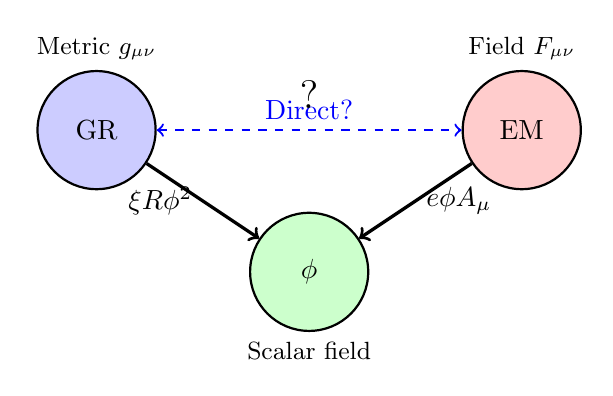
\begin{tikzpicture}[scale=0.9]
    % Coupling diagram showing GR + EM with scalar mediation
    \node[draw,circle,thick,minimum size=1.5cm,fill=blue!20] (gr) at (0,2) {GR};
    \node[draw,circle,thick,minimum size=1.5cm,fill=red!20] (em) at (6,2) {EM};
    \node[draw,circle,thick,minimum size=1.5cm,fill=green!20] (scalar) at (3,0) {$\phi$};

    % Arrows showing coupling
    \draw[->,very thick] (gr) -- (scalar) node[midway,left] {$\xi R\phi^2$};
    \draw[->,very thick] (em) -- (scalar) node[midway,right] {$e\phi A_\mu$};
    \draw[<->,dashed,thick,blue] (gr) -- (em) node[midway,above] {Direct?};

    % Labels
    \node[above,font=\small] at (gr.north) {Metric $g_{\mu\nu}$};
    \node[above,font=\small] at (em.north) {Field $F_{\mu\nu}$};
    \node[below,font=\small] at (scalar.south) {Scalar field};

    % Question mark for direct coupling
    \node[font=\Large] at (3,2.5) {?};
  \end{tikzpicture}
  \caption{Schematic of electromagnetic-gravitational coupling. General relativity (GR) and electromagnetism (EM) may couple directly (blue dashed arrow, unexplored) or through a scalar field mediator $\phi$ (green). Subsequent chapters develop the scalar-mediated unification in detail.}
  \label{fig:p4:coupling-schematic}
\end{figure}

\textbf{Forward to Chapter 2:}

We now develop the mathematical framework of scalar-tensor gravity in detail. Starting from the Brans-Dicke action, we derive complete field equations, analyze conformal transformations between Jordan and Einstein frames, and examine how scalar fields modify gravitational dynamics. Solar system tests and cosmological observations constrain these modifications, setting the stage for electromagnetic coupling in Chapter 3.

\marginnote{The scalar field $\phi$ appearing in Kaluza-Klein and Brans-Dicke will become the central mediator in our unified theory, connecting gravitational curvature to electromagnetic fields.}

%==============================================================================
% END OF CHAPTER 1
%==============================================================================
